\documentclass{beamer}

\usepackage[T1]{fontenc}
\usepackage[utf8]{inputenc}
\usepackage[italian]{babel}
\usepackage{lmodern}
\usepackage{graphicx}

\usetheme[pageofpages=di]{Unipd}

\title{Sviluppo di un sistema web on-premise per la configurazione e il calcolo dei costi di pannelli per l’automazione di valvole industriali}
\subtitle{Esperienza di stage presso Nuvem s.r.l. in collaborazione con Starline Services S.p.A.}
\author[Enrico Cotti Cottini]{Enrico Cotti Cottini}
\date{Luglio 22, 2025}
\institute{Dipartimento di Matematica “Tullio Levi-Civita”\\Corso di Laurea in Informatica\\Università degli Studi di Padova}

% \AtBeginSection[]
% {
%   \begin{frame}
%     \frametitle{Indice}
%     \tableofcontents[currentsection]
%   \end{frame}
% }

\begin{document}

\frame{\titlepage}

% \begin{frame}{Indice}
    % \tableofcontents    
% \end{frame}

% % 2. Azienda ospitante: Nuvem s.r.l.
% \section{Azienda ospitante}
% \begin{frame}{Nuvem s.r.l. - Azienda ospitante}
%     \begin{itemize}
%         \item \textbf{Consulenza IT} e sviluppo software
%         \item \textbf{Innovazione} nei processi aziendali
%         \item \textbf{Ambiente formativo} per lo stage
%         \item \textbf{Team multidisciplinare}
%     \end{itemize}
%     %\includegraphics[width=0.35\textwidth]{nuvem_logo.png}
% \end{frame}

% 3. Azienda cliente: Starline Services S.p.A.
\section{Azienda cliente}
\begin{frame}{Starline S.p.A. - Azienda cliente}
    \begin{itemize}
        \item \textbf{Specializzazione}: valvole a sfera e automazione industriale
        \item \textbf{Divisione Automation}: Starline Automation
        \item \textbf{Focus}: realizzazione di soluzioni per automazione industriale
    \end{itemize}
    %\includegraphics[width=0.35\textwidth]{starline_logo.png}
\end{frame}

% 4. Il sistema attuale: progettazione pannelli in Excel
\section{Sistema attuale}
\begin{frame}{Progettazione pannelli in Excel}
    \begin{itemize}
        \item \textbf{Gestione manuale} tramite fogli Excel
        \item \textbf{Criticità}: errori, lentezza, concorrenza
        \item \textbf{Necessità}: di un sistema centralizzato
    \end{itemize}
    \begin{center}
        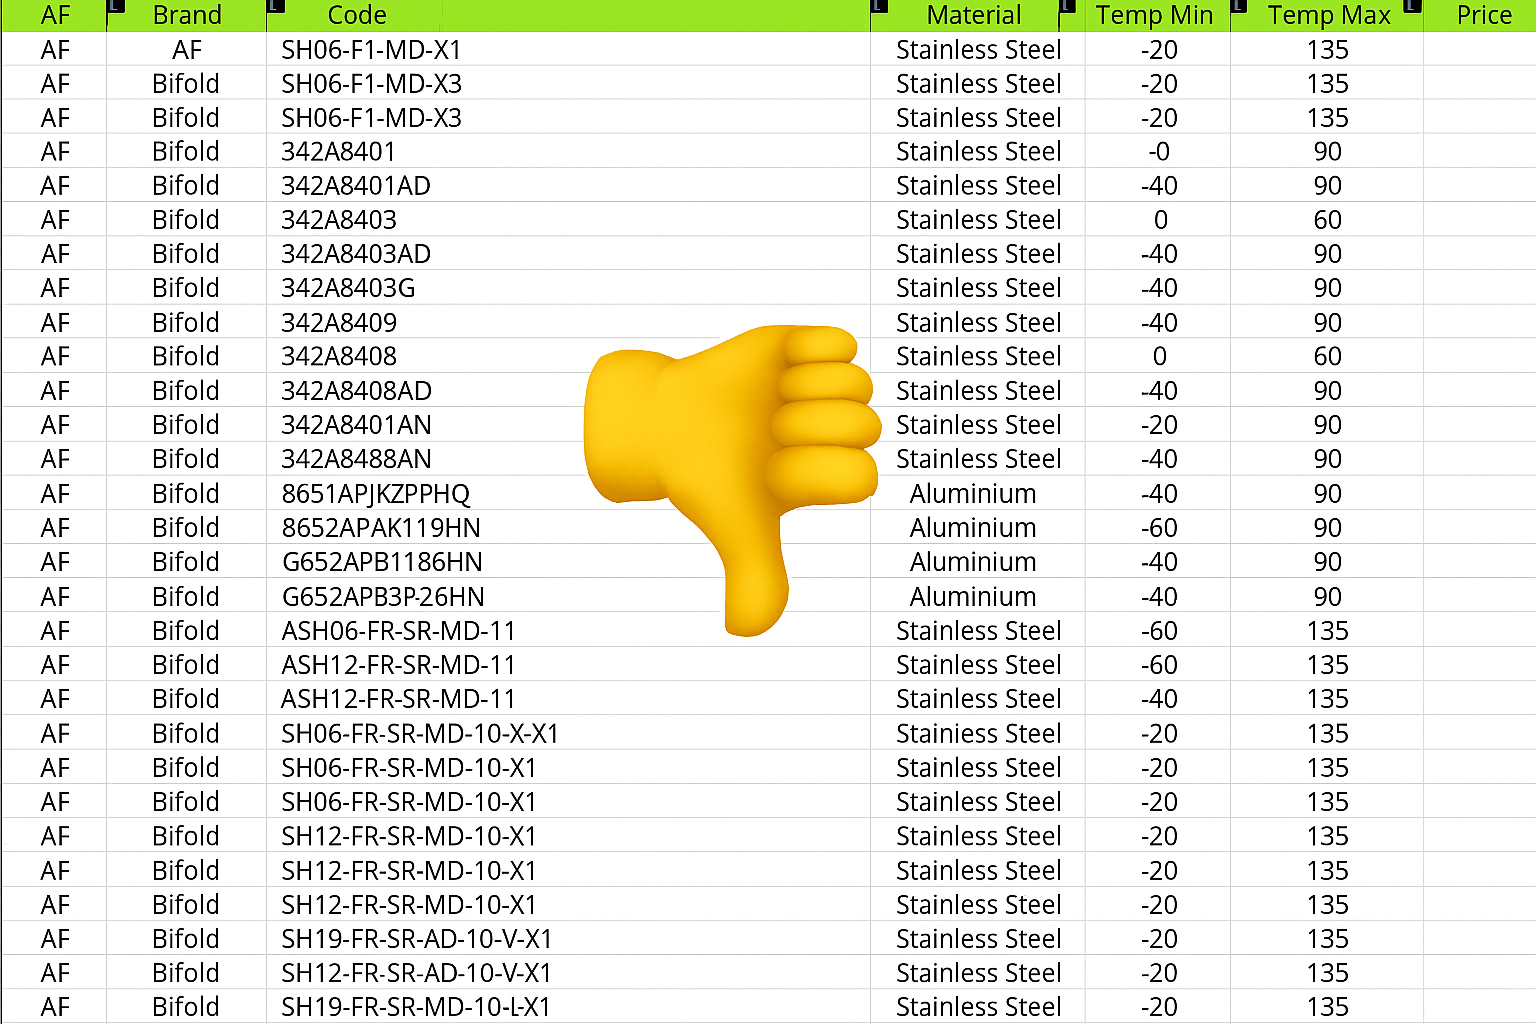
\includegraphics[width=0.5\textwidth]{images/Informazioni prodotto industriale con errore.png} % Sostituisci con l'immagine reale
    \end{center}
\end{frame}

% 5. Contesto applicativo: valvola e attuatore
\section{Contesto applicativo}
\begin{frame}{Valvola e attuatore}
    \begin{itemize}
        \item \textbf{Valvola a sfera}: controllo flusso
        \item \textbf{Attuatore}: apertura/chiusura automatica
    \end{itemize}
    \begin{center}
        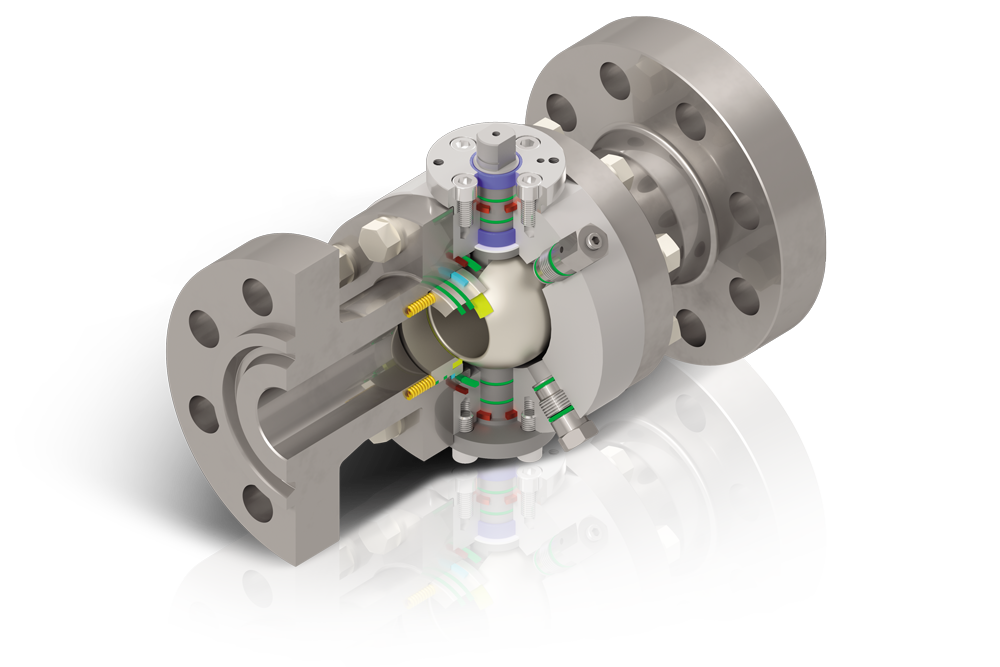
\includegraphics[width=0.45\textwidth]{images/Contesto_Applicativo/valvola_sfera.png}
        \hspace{0.05\textwidth}
        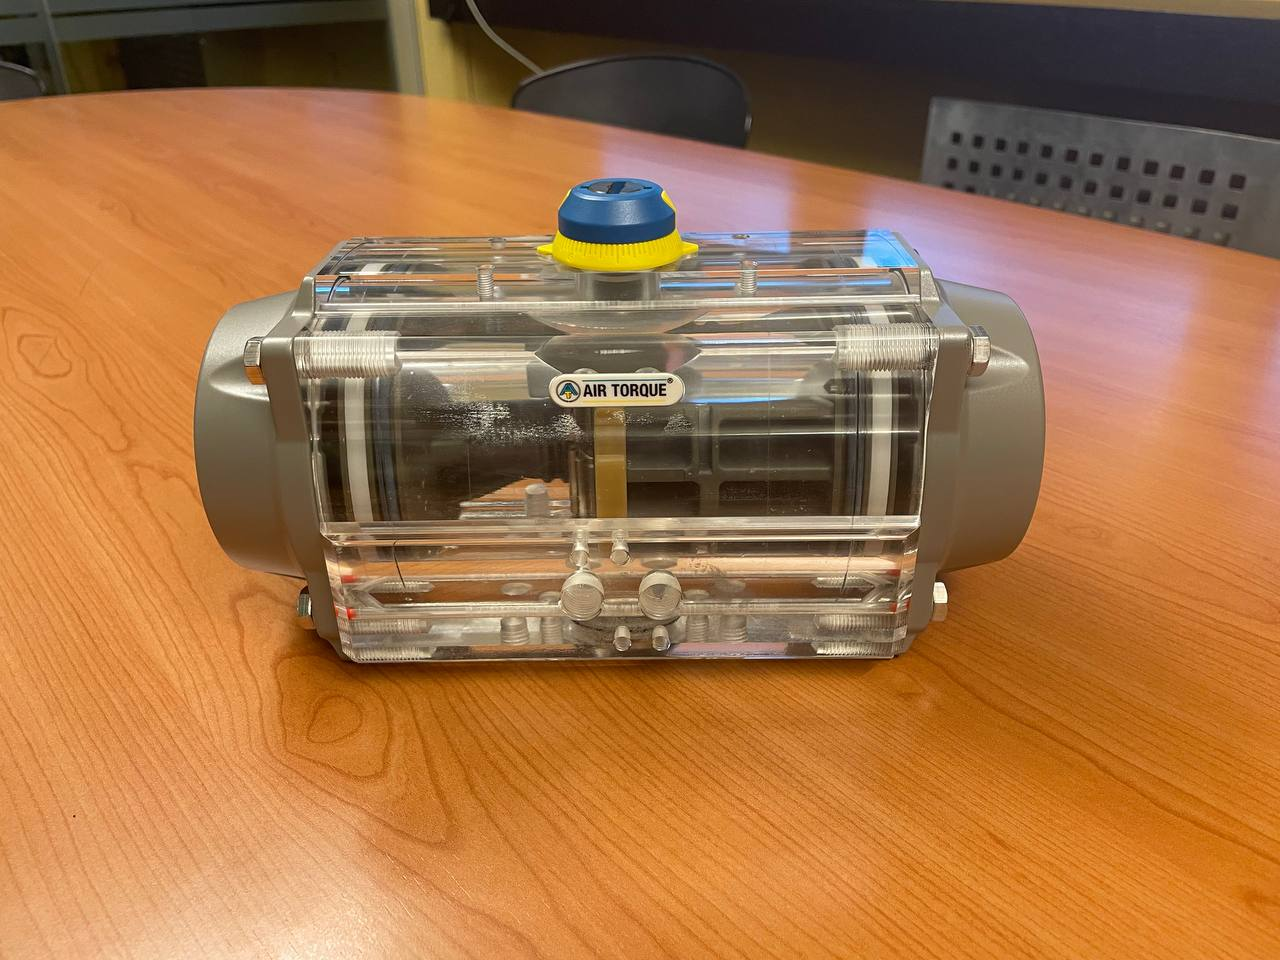
\includegraphics[width=0.45\textwidth]{images/Contesto_Applicativo/attuatore.jpg}
    \end{center}
\end{frame}

% 6. Contesto applicativo: pannello di controllo
\begin{frame}{Pannello di controllo}
    \begin{itemize}
        \item \textbf{Interfaccia} tra operatore e impianto
        \item \textbf{Gestione} attuatori e valvole
        \item \textbf{Personalizzazione} per esigenze cliente
    \end{itemize}
    \begin{center}
        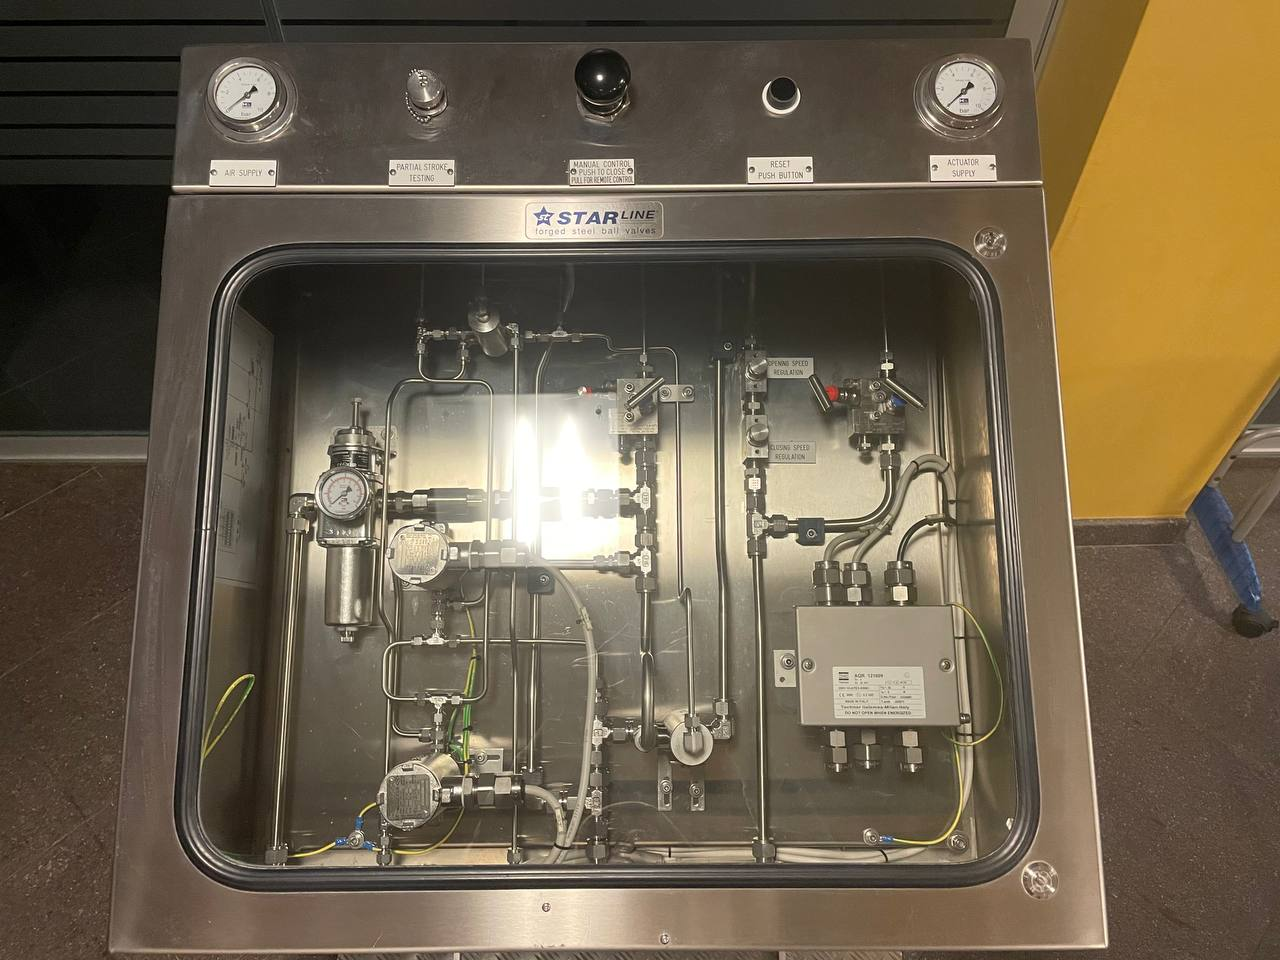
\includegraphics[width=0.6\textwidth]{images/Contesto_Applicativo/pannello_controllo.jpg} % Sostituisci con l'immagine reale
    \end{center}
\end{frame}

% 7. Necessità della soluzione software
\section{Motivazione}
\begin{frame}{Necessità della soluzione software}
    \begin{itemize}
        \item \textbf{Complessità} crescente dei sistemi
        \item \textbf{Limiti} strumenti tradizionali
        \item \textbf{Rischio} di errore umano
        \item \textbf{Centralizzazione} e automazione dati
    \end{itemize}
    %\includegraphics[width=0.5\textwidth]{diagramma_flusso.png}
\end{frame}

% 8. Descrizione dello stage
\section{Stage}
\begin{frame}{Descrizione dello stage}
    \begin{itemize}
        \item \textbf{Durata}: 2 mesi presso Nuvem/Starline
        \item \textbf{Obiettivi}: sviluppo piattaforma, analisi requisiti
        \item \textbf{Ruolo}: analisi, sviluppo
        \item \textbf{Collaborazione} tra cliente e fornitore
    \end{itemize}
\end{frame}

% 9. Metodologia di sviluppo: Agile e Scrum
\section{Metodologia}
\begin{frame}{Metodologia di sviluppo: Agile e Scrum}
    \begin{itemize}
        \item \textbf{Principi} Agile: iterazione, feedback, adattamento
        \item \textbf{Scrum}: ruoli, eventi, artefatti
        \item \textbf{Gestione} del lavoro in team
        \item \textbf{Miglioramento} continuo
    \end{itemize}
    \begin{center}
    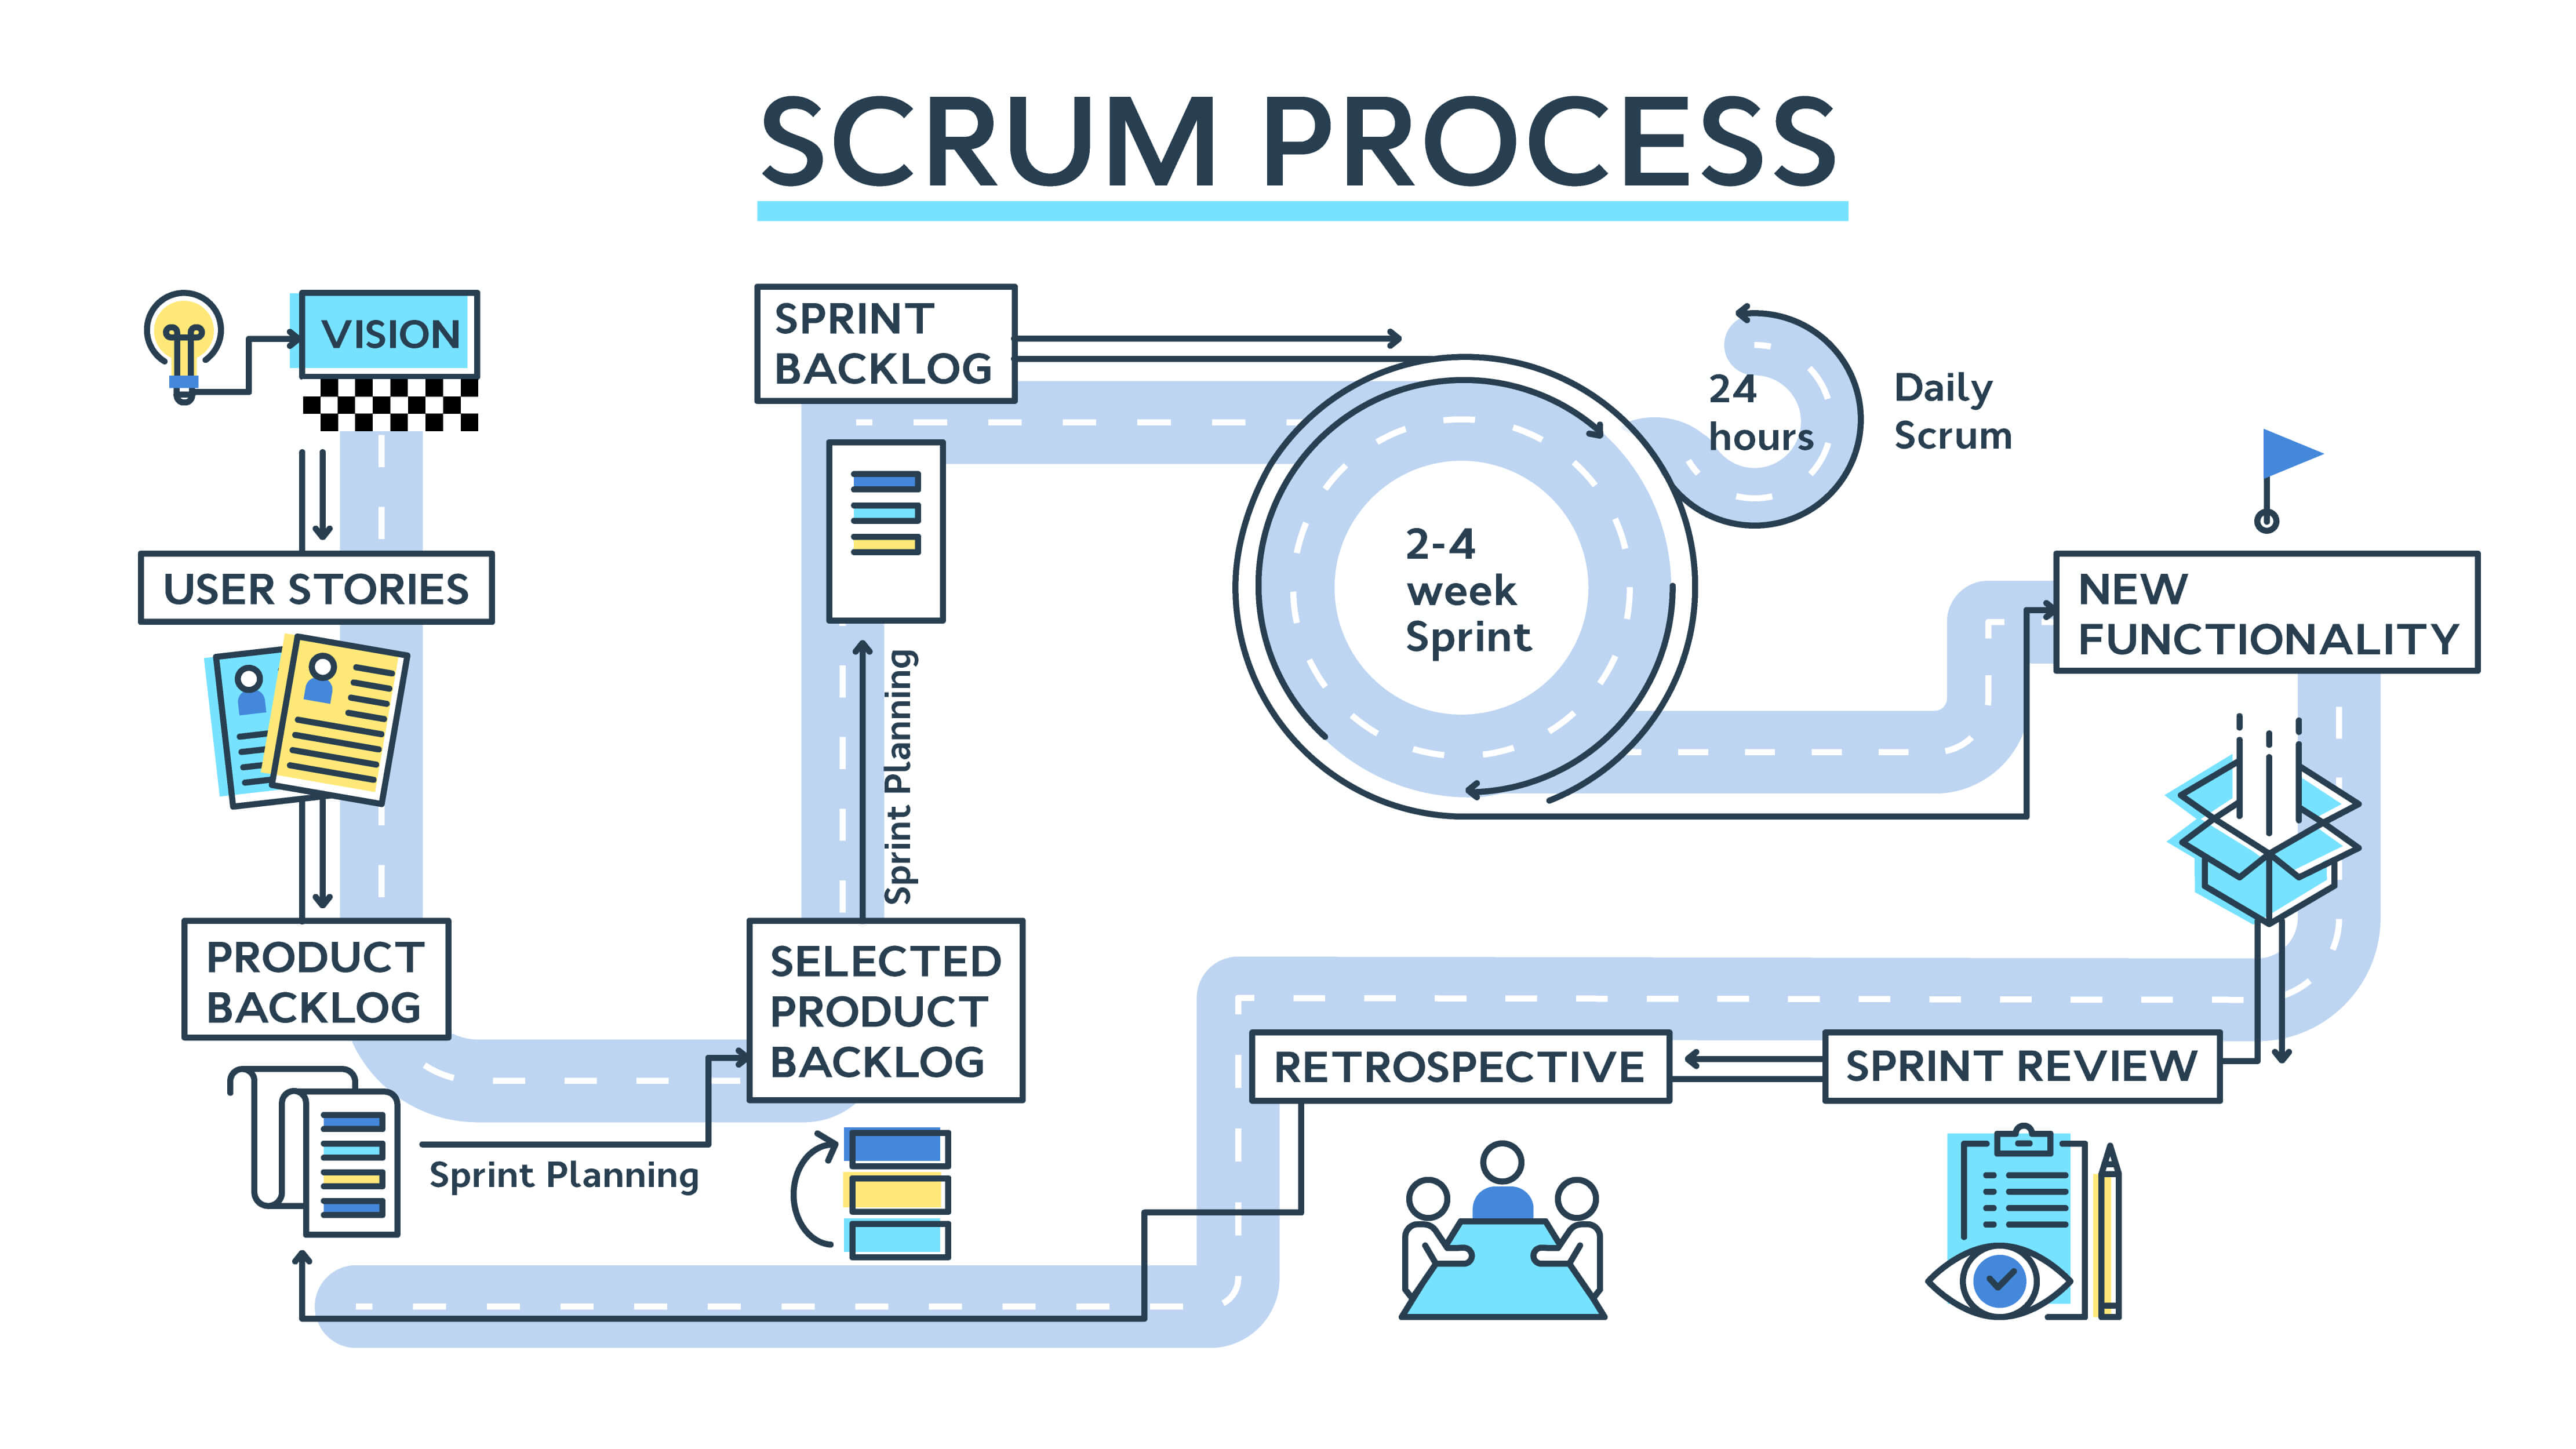
\includegraphics[width=0.7\textwidth]{images/Scrum/scrum-process.jpg}
    \end{center}
\end{frame}

% 10. Scrum applicato al progetto
\begin{frame}{Scrum applicato al progetto}
    \begin{itemize}
        \item \textbf{Adattamento} Scrum al contesto aziendale
        \item \textbf{Strumenti}: GitHub, Teams, Docker
        \item \textbf{Sprint} e review regolari
    \end{itemize}
    %\includegraphics[width=0.4\textwidth]{kanban.png}
\end{frame}

% 11. Analisi dei requisiti
\section{Analisi dei requisiti}
\begin{frame}{Analisi dei requisiti}
    \begin{center}
        \begin{minipage}{0.32\textwidth}
            \centering
            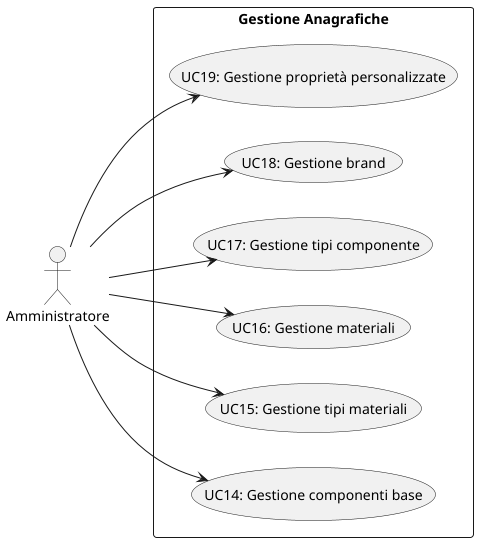
\includegraphics[width=\linewidth]{images/usecase/gestione_anagrafiche.png}\\
        \end{minipage}
        \hfill
        \begin{minipage}{0.50\textwidth}
            \centering
            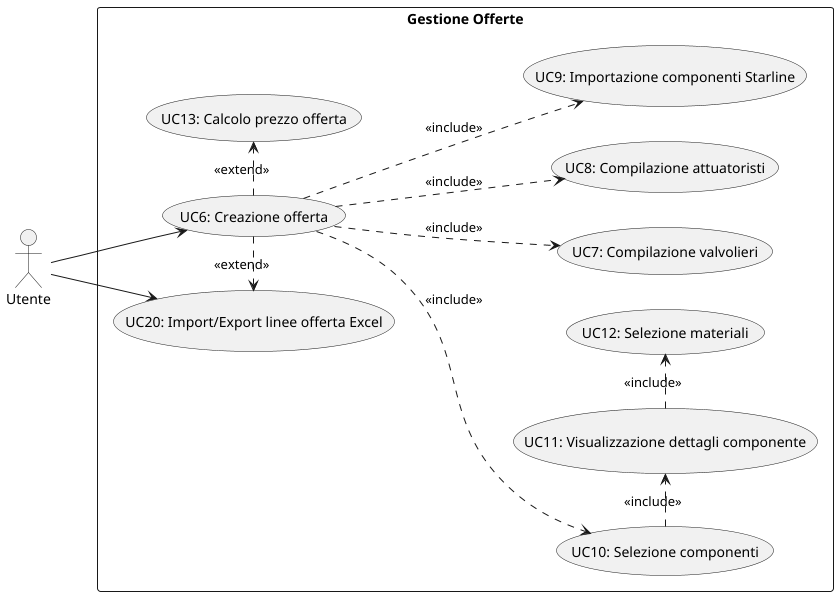
\includegraphics[width=\linewidth]{images/usecase/gestione_offerte.png}\\
        \end{minipage}
        \hfill
        \begin{minipage}{0.50\textwidth}
            \centering
            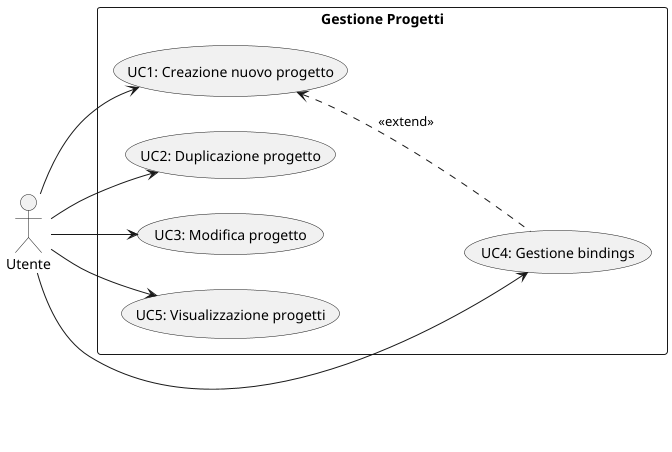
\includegraphics[width=\linewidth]{images/usecase/gestione_progetti.png}\\
        \end{minipage}
    \end{center}
    %\includegraphics[width=0.4\textwidth]{usecase.png}
\end{frame}

% 12. Progettazione: architettura esagonale
\section{Progettazione}
\begin{frame}{Architettura esagonale}
    \begin{center}
    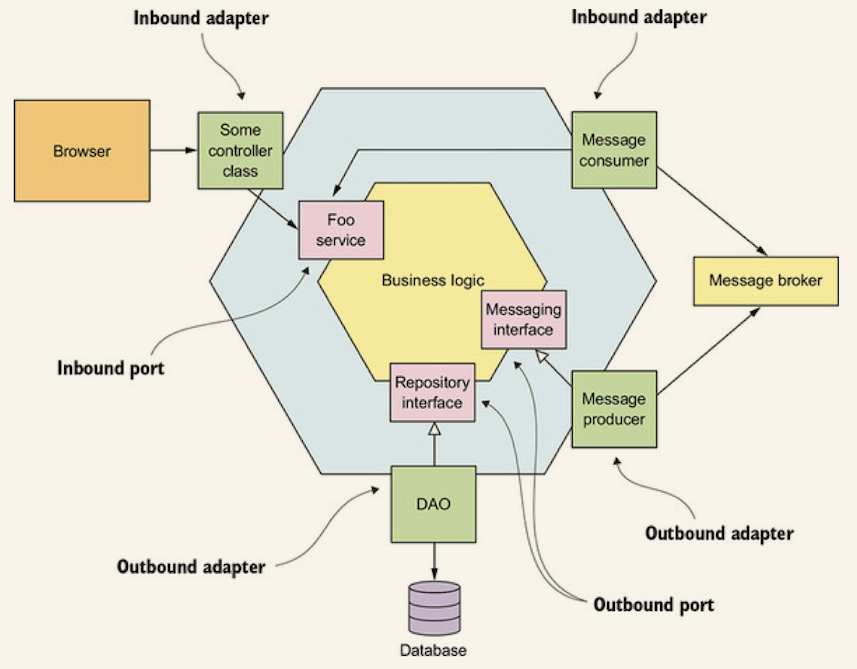
\includegraphics[width=0.8\textwidth]{images/classes/hexagonal-architecture-pattern.png} % Sostituisci con lo schema reale
    \end{center}
\end{frame}

% 13. Progettazione: dependency injection
\begin{frame}{Dependency Injection}
    \begin{itemize}
        \item \textbf{Gestione automatica} delle dipendenze
        \item \textbf{Modularità} e riusabilità del codice
        \item \textbf{Implementazione} tramite framework .NET
    \end{itemize}
    %\includegraphics[width=0.45\textwidth]{dependency_injection.png} % Schema o snippet di codice
\end{frame}

% 14. Progettazione e tecnologie
\begin{frame}{Tecnologie e frontend}
    \begin{itemize}
        \item \textbf{MudBlazor}: interfaccia web moderna in Blazor
        \item \textbf{Scalar}:  interfaccia interattiva per test API 
        \item \textbf{MongoDB}: database NoSQL flessibile
        \item \textbf{Docker}: containerizzazione e portabilità
        \item \textbf{Rider}: IDE avanzato per lo sviluppo .NET
    \end{itemize}
    %\includegraphics[width=0.45\textwidth]{frontend.png} % Screenshot UI o diagramma tecnico
\end{frame}


\begin{frame}{Conclusioni e prospettive}
    \begin{itemize}
        \item \textbf{Benefici ottenuti}: velocità, tracciabilità, riduzione degli errori
        \item \textbf{Criticità}: alcune funzionalità avanzate ancora da completare
        \item \textbf{Prospettive}: ottimizzazione Interfaccia, gestione ruoli, integrazione API
        \item \textbf{Esperienza formativa} in contesto reale
    \end{itemize}
    %\includegraphics[width=0.35\textwidth]{ringraziamenti.png}
\end{frame}

 
% Slide finale
\begin{emptyframe}
    \centering
    \textbf{Grazie per l'attenzione!}
\end{emptyframe}

\end{document}